\documentclass[11pt]{article}

\usepackage[margin=0.5in]{geometry}
\usepackage{graphicx}
\usepackage{subcaption}
\usepackage{caption}

\begin{document}

\begin{itemize}
\item $\epsilon$ is maximum value for $L^\infty$ error
\item Best tested $\epsilon$ used to reach convergence for each test
\item Including new nodes as average of surrounding values or as big value does not effect results
\item Locking unrefined nodes in AMR moderately increases $L^1$ error, but reduces computation time
\item All elements associated with refinement node are refined
\item Each element divided into 4 triangles when refined (conformal adaptation)
\item First order sweeping from Qian, Zhang, and Zhao (2007)
\end{itemize}

\section*{Two-circle problem}

\begin{table}[h!]
\begin{center}
\begin{tabular}{|r|r|c|c|r|}
\hline
Nodes & Elements & $L^1$ error & $L^\infty$ error & CPU (sec) \\
\hline
64 & 104 & $1.85 \times 10^{-1}$ & $6.73 \times 10^{-1}$ & 0.13 \\
233 & 416 & $1.02 \times 10^{-1}$ & $7.24 \times 10^{-1}$ & 0.81 \\
881 & 1664 & $2.71 \times 10^{-2}$ & $1.27 \times 10^{-1}$ & 3.32 \\
3425 & 6656 & $6.51 \times 10^{-3}$ & $2.86 \times 10^{-2}$ & 19.51 \\
13505 & 26624 & $2.45 \times 10^{-3}$ & $1.41 \times 10^{-2}$ & 102.41 \\
53633 & 106496 & $1.20 \times 10^{-3}$ & $8.46 \times 10^{-3}$ & 744.63 \\
\hline
\end{tabular}
\end{center}
\caption{Acute triangulation, spherical wave sweeping based on $l^2$-metric ordering, 4 corners as reference, both ascent and descent orderings}
\end{table}

% \begin{table}[h!]
% \begin{center}
% \begin{tabular}{|r|r|r|r|c|c|c|r|}
% \hline
% Initial nodes & Initial elements & Final nodes & Fianl elements & $\epsilon$ & $L^1$ error & $L^\infty$ error & CPU (sec) \\
% \hline
% 64 & 104 & 2018 & 3902 & $3.2 \times 10^{-2}$ & $1.16 \times 10^{-2}$ & $3.16 \times 10^{-2}$ & 15.74 \\
% 233 & 416 & 2018 & 3902 & $3.2 \times 10^{-2}$ & $1.16 \times 10^{-2}$ & $3.16 \times 10^{-2}$ & 15.29 \\
% 881 & 1664 & 2252 & 4368 & $3.3 \times 10^{-2}$ & $1.14 \times 10^{-2}$ & $3.28 \times 10^{-2}$ & 16.41 \\
% 3425 & 6656 & 3543 & 6892 & $2.2 \times 10^{-2}$ & $6.23 \times 10^{-3}$ & $2.18 \times 10^{-2}$ & 26.79 \\
% \hline
% \end{tabular}
% \end{center}
% \caption{Acute initial triangulation, no obtuse treatment, AMR, locking old nodes, averaging new nodes, spherical wave sweeping based on $l^2$-metric ordering, 4 corners as reference, both ascent and descent orderings}
% \end{table}
%
% \begin{table}[h!]
% \begin{center}
% \begin{tabular}{|r|r|r|r|c|c|c|r|}
% \hline
% Initial nodes & Initial elements & Final nodes & Fianl elements & $\epsilon$ & $L^1$ error & $L^\infty$ error & CPU (sec) \\
% \hline
% 64 & 104 & 1966 & 3802 & $3.6 \times 10^{-2}$ & $8.22 \times 10^{-3}$ & $3.54 \times 10^{-2}$ & 20.44 \\
% 233 & 416 & 1966 & 3802 & $3.6 \times 10^{-2}$ & $8.22 \times 10^{-3}$ & $3.54 \times 10^{-2}$ & 20.30 \\
% 881 & 1664 & 2190 & 4244 & $3.6 \times 10^{-2}$ & $7.70 \times 10^{-3}$ & $3.54 \times 10^{-2}$ & 33.47 \\
% 3425 & 6656 & 3543 & 6892 & $2.2 \times 10^{-2}$ & $5.82 \times 10^{-3}$ & $2.18 \times 10^{-2}$ & 45.08 \\
% \hline
% \end{tabular}
% \end{center}
% \caption{Acute initial triangulation, no obtuse treatment, AMR, averaging new nodes, spherical wave sweeping based on $l^2$-metric ordering, 4 corners as reference, both ascent and descent orderings}
% \end{table}

\begin{table}[h!]
\begin{center}
\begin{tabular}{|r|r|r|r|c|c|c|r|}
\hline
Initial nodes & Initial elements & Final nodes & Final elements & $\epsilon$ & $L^1$ error & $L^\infty$ error & CPU (sec) \\
\hline
64 & 104 & 1986 & 3840 & $3.6 \times 10^{-2}$ & $1.21 \times 10^{-2}$ & $3.49 \times 10^{-2}$ & 13.59 \\
233 & 416 & 1986 & 3840 & $3.6 \times 10^{-2}$ & $1.21 \times 10^{-2}$ & $3.49 \times 10^{-2}$ & 13.00 \\
881 & 1664 & 2178 & 4220 & $3.6 \times 10^{-2}$ & $1.15 \times 10^{-2}$ & $3.52 \times 10^{-2}$ & 13.40 \\
3425 & 6656 & 3543 & 6892 & $2.2 \times 10^{-2}$ & $6.23 \times 10^{-3}$ & $2.18 \times 10^{-2}$ & 21.47 \\
\hline
\end{tabular}
\end{center}
\caption{Acute initial triangulation, one iteration of obtuse treatment, AMR, locking old nodes, averaging new nodes, spherical wave sweeping based on $l^2$-metric ordering, 4 corners as reference, both ascent and descent orderings}
\end{table}

\begin{table}[h!]
\begin{center}
\begin{tabular}{|r|r|r|r|c|c|c|r|}
\hline
Initial nodes & Initial elements & Final nodes & Final elements & $\epsilon$ & $L^1$ error & $L^\infty$ error & CPU (sec) \\
\hline
64 & 104 & 1840 & 3558 & $3.9 \times 10^{-2}$ & $7.75 \times 10^{-3}$ & $3.52 \times 10^{-2}$ & 14.14 \\
233 & 416 & 1846 & 3570 & $3.9 \times 10^{-2}$ & $7.75 \times 10^{-3}$ & $3.52 \times 10^{-2}$ & 13.51 \\
881 & 1664 & 2166 & 4196 & $3.6 \times 10^{-2}$ & $7.66 \times 10^{-3}$ & $3.46 \times 10^{-2}$ & 19.83 \\
3425 & 6656 & 3543 & 6892 & $2.2 \times 10^{-2}$ & $5.82 \times 10^{-3}$ & $2.17 \times 10^{-2}$ & 36.82 \\
\hline
\end{tabular}
\end{center}
\caption{Acute initial triangulation, one iteration of obtuse treatment, AMR, averaging new nodes, spherical wave sweeping based on $l^2$-metric ordering, 4 corners as reference, both ascent and descent orderings}
\end{table}

\newpage

\begin{figure}
  \centering
  \begin{subfigure}[b]{0.45\textwidth}
    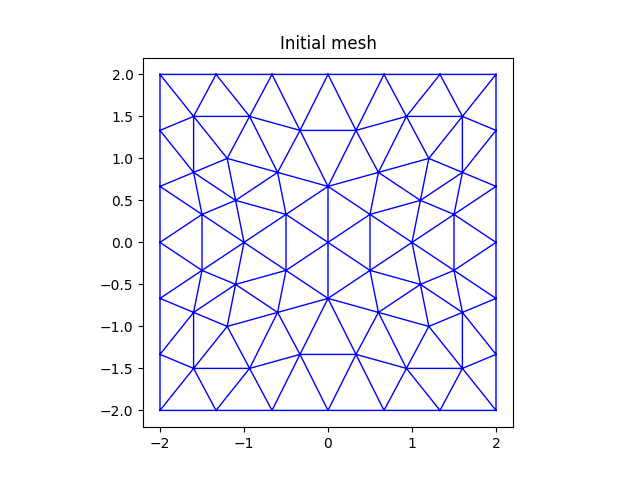
\includegraphics[scale=0.6]{grid.png}
    \caption{Acute triangulation, 64 nodes, 104 elements}
  \end{subfigure}
  \begin{subfigure}[b]{0.45\textwidth}
    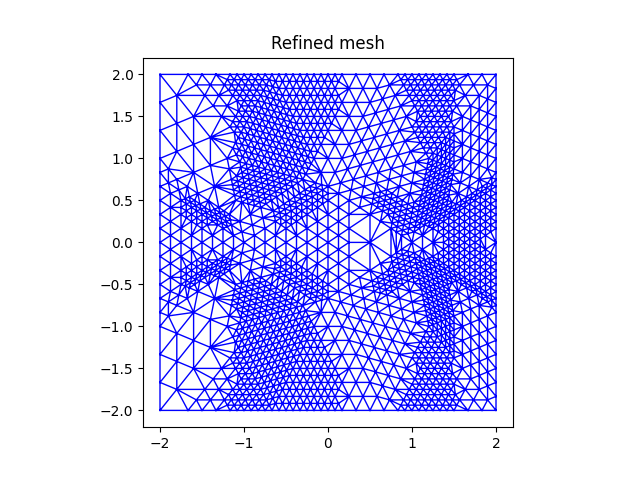
\includegraphics[scale=0.6]{grid_refined.png}
    \caption{Adaptively refined mesh, 1840 nodes, 3558 elements}
  \end{subfigure}
  \begin{subfigure}[b]{0.45\textwidth}
    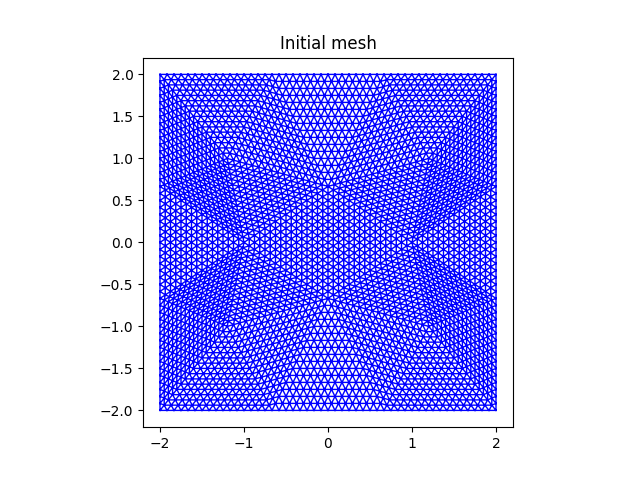
\includegraphics[scale=0.6]{grid-fine.png}
    \caption{Acute triangulation, 3425 nodes, 6656 elements}
  \end{subfigure}
\end{figure}

\newpage

\begin{figure}
  \centering
  \begin{subfigure}[b]{0.45\textwidth}
    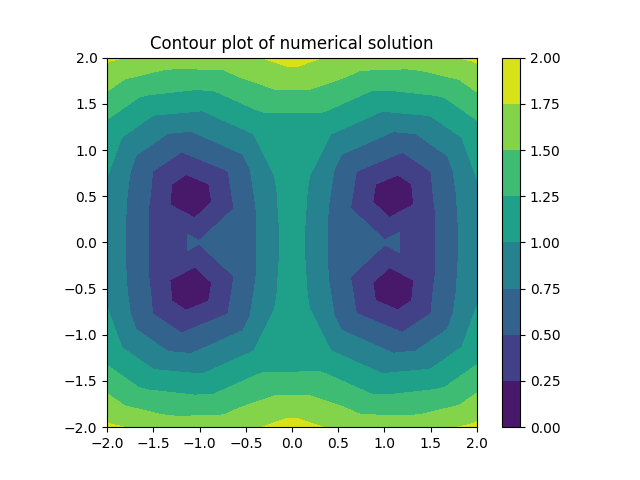
\includegraphics[scale=0.6]{solution.png}
    \caption{Standard solution, 64 nodes, 104 elements}
  \end{subfigure}
  \begin{subfigure}[b]{0.45\textwidth}
    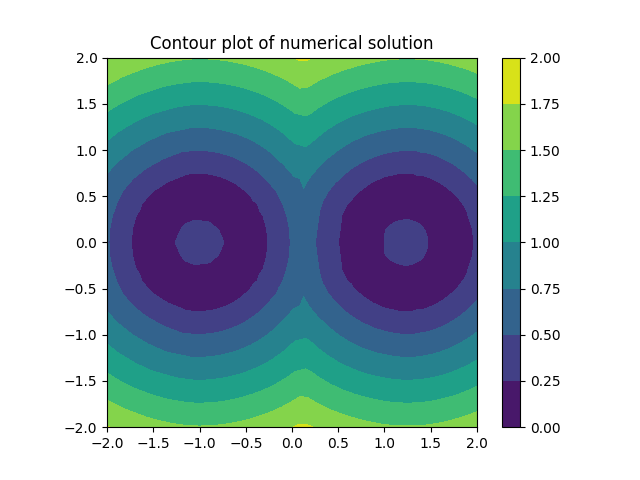
\includegraphics[scale=0.6]{AMRsolution.png}
    \caption{AMR solution, 1840 nodes, 3558 elements, no locking}
  \end{subfigure}
  \begin{subfigure}[b]{0.45\textwidth}
    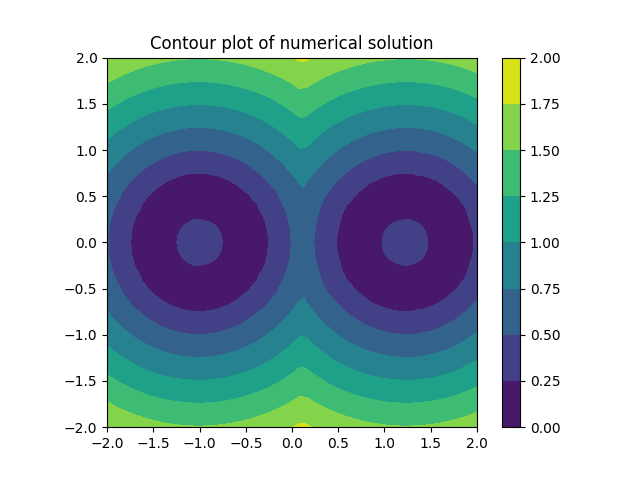
\includegraphics[scale=0.6]{solution-refined.png}
    \caption{Standard solution, 3425 nodes, 6656 elements}
  \end{subfigure}
\end{figure}

\end{document}
